%%
%% Modified by Ricardo Garcia-Rosas to satisfy the rules established by the University of Melbourne's Research Higher Degrees Committee as of 4th of June 2019.
%% Guidelines can be found at: https://gradresearch.unimelb.edu.au/__data/assets/pdf_file/0004/2027839/Preparation-of-GR-theses-rules.pdf
%%
%%%%%%%%%%%%%%%%%%%%%%%%%%%%%%%%%%%%%%%%%%%%%%%%%%%%%%%%%%%%%%%%%%%%%%%%%
%% IMPORTANT NOTE TO AUTHOR:
%% As part of the guidelines, the use of the university logo is not permitted. This template contains it to make it easier to find/recognise in the Overleaf Gallery. To make the template compliant please go to 'Thesis.cls' and comment out the \includegraphics command in line 217 (it is clearly highlited).
%%%%%%%%%%%%%%%%%%%%%%%%%%%%%%%%%%%%%%%%%%%%%%%%%%%%%%%%%%%%%%%%%%%%%%%%%
%%
%% ----------------------------------------------------------------
%% Thesis.tex -- MAIN FILE (the one that you compile with LaTeX)
%% ---------------------------------------------------------------- 

% Set up the document
\documentclass[a4paper, 11pt, oneside]{Thesis}  % Use the "Thesis" style, based on the ECS Thesis style by Steve Gunn
%
% Put your figures in this directory
\graphicspath{Figures/}  % Location of the graphics files (set up for graphics to be in PDF format)
%

% Include any extra LaTeX packages required
\usepackage[square, numbers, comma, sort&compress]{natbib}  % Use the "Natbib" style for the references in the Bibliography
\usepackage{verbatim}  % Needed for the "comment" environment to make LaTeX comments
\usepackage{vector}  % Allows "\bvec{}" and "\buvec{}" for "blackboard" style bold vectors in maths
% Packages and macros used by this report
\usepackage{lmodern}  % vector Computer Modern (the template font)
\usepackage[T1]{fontenc}
\usepackage{tabularx}
\usepackage{array}
\usepackage{xurl}
\usepackage{enumitem}
\usepackage{placeins}
\newcommand{\lab}[1]{\textsc{#1}}  % evidence labels
\newcommand{\Fmax}{\ensuremath{F_{\max}}}
\newcommand{\by}{\ensuremath{\times}}
\newcommand{\ra}{\ensuremath{\rightarrow}}
\newcolumntype{L}[1]{>{\raggedright\arraybackslash}p{#1}}
\newcolumntype{Y}{>{\raggedright\arraybackslash}X}
\hypersetup{urlcolor=blue, colorlinks=true}  % Colours hyperlinks in blue, but this can be distracting if there are many links.

%% ----------------------------------------------------------------
\begin{document}
\frontmatter      % Begin Roman style (i, ii, iii, iv...) page numbering

%
\UNIVERSITY{{THE UNIVERSITY OF MELBOURNE }}    
%
%%%%%%%%%%%%%%%%%%%%%%%%%%%%%%%%%%%%%%%%%%%%%%%%%%%%%%%%%%%%%%%%%%%%%%%%%
% Update your department and school here:
\department{{School of Computing and Information Systems}}
\school{{Faculty of Engineering and Information Technology}}
%%%%%%%%%%%%%%%%%%%%%%%%%%%%%%%%%%%%%%%%%%%%%%%%%%%%%%%%%%%%%%%%%%%%%%%%%

%
%%%%%%%%%%%%%%%%%%%%%%%%%%%%%%%%%%%%%%%%%%%%%%%%%%%%%%%%%%%%%%%%%%%%%%%%%
% Set up the Title Page
% Change your thesis title and your information here
\title  {Herded or Anchored? Testing Conformity in Machine Learning on a Decade of ICLR Submissions}
\authors  {Minghan Li}
\degree   {A report submitted for\\ Science Research Project (SCIE30001)\\[1ex] Supervisor: A/Prof Jianzhong Qi}
\addresses  {\groupname\\\deptname\\\univname}  % Do not change this here, instead these must be set in the "Thesis.cls" file, please look through it instead
\date       {\today}
\subject    {}
\keywords   {}
%%%%%%%%%%%%%%%%%%%%%%%%%%%%%%%%%%%%%%%%%%%%%%%%%%%%%%%%%%%%%%%%%%%%%%%%%

\maketitle
%% ----------------------------------------------------------------

\setstretch{1.3}  % It is better to have smaller font and larger line spacing than the other way round

% Define the page headers using the FancyHdr package and set up for one-sided printing
\fancyhead{}  % Clears all page headers and footers
\rhead{\thepage}  % Sets the right side header to show the page number
\lhead{}  % Clears the left side page header

\pagestyle{fancy}  % Finally, use the "fancy" page style to implement the FancyHdr headers

%% ----------------------------------------------------------------
% The Abstract Page

\addtotoc{Abstract}  % Add the "Abstract" page entry to the Contents
\abstract{
\addtocontents{toc}{\vspace{1em}}  % Add a gap in the Contents, for aesthetics

Machine learning is often said to herd: researchers chase what is popular, and peer review rewards them for it. But a
field can converge without copying. Researchers may instead stay close to a record: their own earlier work, or a topic
they already know. We call these two routes to conformity \emph{imitation} and \emph{continuity}, and test the herding
account where they make different predictions. The data are 43,480 ICLR submissions from 2017 to 2026, including
rejected and withdrawn papers; hypotheses were registered before any outcome was examined and re-tested on 11,099
held-out papers. The field did converge on foundation models, but both routes predict this, and the number of topics
that appear to be emerging depends on hindsight: between 8 and 29, depending on which years the topic model is fitted
to. Where the two routes make different predictions, we find no evidence of herding. Researchers new to a topic propose
methods more often than incumbents do, the reverse of our registered prediction. At review, acceptance shows no detectable difference for papers in crowded topics, whereas papers far from their authors' earlier work are accepted less often
(a post hoc finding, confirmed on held-out papers). The conformity visible at ICLR is anchored to researchers' own
records rather than driven by the crowd.

}

\clearpage  % Abstract ended, start a new page

%% ----------------------------------------------------------------
% Declaration Page required for the Thesis, your institution may give you a different text to place here
%
% Guidelines as of 2019/06/04
% https://gradresearch.unimelb.edu.au/__data/assets/pdf_file/0004/2027839/Preparation-of-GR-theses-rules.pdf
%
\Declaration{

\addtocontents{toc}{\vspace{1em}}  % Add a gap in the Contents, for aesthetics

I, Minghan Li, declare that this report titled, `Herded or Anchored? Testing Conformity in Machine Learning on a Decade of ICLR Submissions' and the work presented in it are my own. I confirm that:

\begin{itemize} 
\item[\tiny{$\blacksquare$}] The report comprises only my original work towards Science Research Project (SCIE30001) except where indicated in the preface;
 
\item[\tiny{$\blacksquare$}] due acknowledgement has been made in the text to all other material used; and

\item[\tiny{$\blacksquare$}] the report is within the word limit set for it, exclusive of tables, maps, bibliographies and appendices.
\\
\end{itemize}
 
 
Signed:\\
\rule[1em]{25em}{0.5pt}  % This prints a line for the signature
 
Date:\\
\rule[1em]{25em}{0.5pt}  % This prints a line to write the date
}
\clearpage  % Declaration ended, now start a new page

%% ----------------------------------------------------------------
% Preface Page required for the Thesis, your institution may give you a different text to place here
%
% Guidelines as of 2019/06/04
% https://gradresearch.unimelb.edu.au/__data/assets/pdf_file/0004/2027839/Preparation-of-GR-theses-rules.pdf
%
\Preface{

\addtocontents{toc}{\vspace{1em}}  % Add a gap in the Contents, for aesthetics

This report is the author's own work for Science Research Project (SCIE30001), carried out under the supervision of A/Prof Jianzhong Qi. It has not been submitted for another qualification and is unpublished material not submitted for publication.

}
\clearpage  % Preface ended, now start a new page

%% ----------------------------------------------------------------
% The Acknowledgements page, for thanking everyone
\setstretch{1.3}  % Reset the line-spacing to 1.3 for body text (if it has changed)
\acknowledgements{
\addtocontents{toc}{\vspace{1em}}  % Add a gap in the Contents, for aesthetics

I thank my supervisor, A/Prof Jianzhong Qi, for guidance and feedback throughout this project.

}
\clearpage  % End of the Acknowledgements
%% ----------------------------------------------------------------

\pagestyle{fancy}  %The page style headers have been "empty" all this time, now use the "fancy" headers as defined before to bring them back


%% ----------------------------------------------------------------
\lhead{\emph{Contents}}  % Set the left side page header to "Contents"
\tableofcontents  % Write out the Table of Contents

%% ----------------------------------------------------------------
\lhead{\emph{List of Figures}}  % Set the left side page header to "List if Figures"
\listoffigures  % Write out the List of Figures

%% ----------------------------------------------------------------
\lhead{\emph{List of Tables}}  % Set the left side page header to "List of Tables"
\listoftables  % Write out the List of Tables

%% ----------------------------------------------------------------
\setstretch{1.5}  % Set the line spacing to 1.5, this makes the following tables easier to read
\clearpage  % Start a new page
\lhead{\emph{Abbreviations}}  % Set the left side page header to "Abbreviations"
\listofsymbols{ll}  % Include a list of Abbreviations (a table of two columns)
{
% \textbf{Acronym} & \textbf{W}hat (it) \textbf{S}tands \textbf{F}or \\
\textbf{CI} & Confidence interval (95\% unless stated) \\
\textbf{FE} & Fixed effects \\
\textbf{FM} & Foundation model \\
\textbf{ICLR} & International Conference on Learning Representations \\
\textbf{LLM} & Large language model \\
\textbf{MDE80} & Minimum detectable effect at 80\% power \\
\textbf{pp} & Percentage points \\

}

%% ----------------------------------------------------------------
\clearpage  %Start a new page
\lhead{\emph{Symbols}}  % Set the left side page header to "Symbols"
\listofnomenclature{lll}  % Include a list of Symbols (a three column table)
{
% symbol & name & unit \\
$F_{\max}$ & closeness to the team's earlier ICLR work & cosine \\
$b$ & slope of later topic edges on earlier ones & -- \\
$k$ & number of topics in a topic map & -- \\
$\kappa$ & agreement between two labelling passes & -- \\
}
%% ----------------------------------------------------------------
% End of the pre-able, contents and lists of things


%% ----------------------------------------------------------------
\mainmatter	  % Begin normal, numeric (1,2,3...) page numbering
\pagestyle{fancy}  % Return the page headers back to the "fancy" style

% Include the chapters of the thesis, as separate files
% Just uncomment the lines as you write the chapters

\chapter{Introduction}
\label{sec:intro}
\lhead{\emph{Chapter 1. Introduction}}  % page header

\begin{figure}[t]
  \centering
  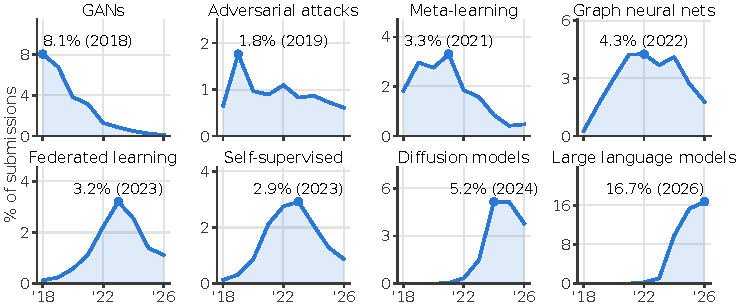
\includegraphics[width=\textwidth]{figs/fig1_waves.pdf}
  \caption[Research waves at ICLR, 2018--2026]{Research waves at ICLR: share of discovery submissions listing each author keyword, 2018--2026; dots
  mark the peak. The eight keywords were chosen for display after their curves were known. Across the 68 most
  frequent keywords, 17 peaked in 2019--2024 with shares of at most half the peak both before it and in 2026.
  Uses no acceptance data.}
  \label{fig:waves}
\end{figure}

Machine learning is often said to herd. Between 2017 and 2026, yearly submissions to the International Conference
on Learning Representations (ICLR) in our discovery corpus grew 40-fold, from 384 to 15,411. The share building on a
foundation model (FM) rose from 0.3\% to 54.4\%, and the share proposing a new architecture fell from 24.5\% to
7.5\%. Keywords rose and fell (Figure~\ref{fig:waves}): generative adversarial networks fell from 8.1\% of
submissions in 2018, and large language models reached 16.7\% in 2026. The wave is NLP's too, as its researchers
increasingly publish at ML venues \citep{jurgens2026future}. Whether science has fashions is an old question
\citep{crane1969fashion}. Critics of ML scholarship point to incentives that favour short-term success
\citep{lipton2019troubling} and to convergence on what suits the field's hardware, benchmarks and foundation models
\citep{hooker2021hardware,dehghani2021benchmark,bommasani2021opportunities}; cascade and fashion theories explain
waves by people taking their cue from others
\citep{bikhchandani1992theory,banerjee1992simple,abrahamson1991managerial}.

Is the switch to FMs not herding enough? Convergence on a shared substrate is
predicted by lock-in, by the efficient choice of a tool that works and by a bandwagon alike, so the curve cannot tell
them apart. The herding question is about behaviour: what researchers write when they enter a topic, and what the
review gate accepts. There, two routes to conformity part. \emph{Imitation} takes its reference point from what
others are doing now: what is popular, rising or recently accepted. \emph{Continuity} takes it from a record: the
team's own earlier work, or a topic that a team member already knows. Imitation makes teams alike; continuity keeps
each team near its own past. We call work that conforms by continuity \emph{anchored}.\footnote{`Anchored' names a position relative to a record, not a mechanism.
It is not the anchoring-and-adjustment heuristic \citep{tversky1974judgment}, the sense in which writing on herding
in science uses the word \citep{baddeley2015herding}.}

Read as herding, the waves make three claims: they are fashions; newcomers to a topic carry them by following
others; and review favours following. We test each claim at its site, the field, entry to a topic and the
acceptance gate, on 43,480 ICLR submissions from 2017--2026, rejected and withdrawn papers included. Hypotheses
were registered before any full-corpus label existed, outcomes stayed sealed until one frozen run, and the main tests were run again on 11,099 held-out papers: a pre-registered out-of-sample replication, not a
certified untouched holdout. Each finding carries one of three labels: \lab{replicated} (from a registered test,
supported again on held-out papers), \lab{held-out supported} (found post hoc, then supported by a
test declared before the held-out data were read) or \lab{exploratory} (discovery only, or descriptive). Tests
without a verdict are called inconclusive or uninformative (Chapter~\ref{sec:design}).

At the field level, keyword waves are real, but emergence depends on hindsight, and the durable shift, the FM
package, fits every route. At entry, researchers new to a topic propose methods more often than incumbents, while,
in the FM era, benchmark and evaluation work sits with incumbents: the opposite of the follow-on entry that herding
implies, and of our own registered prediction. At the gate, no premium for crowded topics is detectable, the branded
title's small premium lies below what the held-out test could detect, and what replicated, apart from regressing
topic edges, is tied to the team's own record.

Prior work relates ICLR acceptance to prestige, process and research area
\citep{tran2020open,ibrahim2026bias,jung2025what,wang2023what,xu2026reviewer} and describes which papers start
topics, who enters LLM research and how far researchers move from their own past work
\citep{huang2026catalyst,movva2024topics,bao2025persistence}. To our knowledge, among the works we checked, none
tests the herding account at entry and at the gate within one submission population, with registered hypotheses
re-tested on held-out papers, as \citet{ibrahim2026bias} did for a prestige gap. We contribute:
\begin{itemize}[leftmargin=*,itemsep=1pt,topsep=3pt,parsep=0pt]
\item \textbf{Entry.} A registered test of herding where imitation predicts it most sharply. Researchers entering a
topic propose methods more often (+3.7\,pp; \lab{replicated}). The surplus holds for researchers with ICLR work in
other topics and predates the FM wave, while, in the FM era, benchmark and evaluation work sits with topic
incumbents and larger teams (\lab{exploratory}).
\item \textbf{Gate.} Using every decided submission under double-blind review, rejected ones included, acceptance
goes with closeness to the team's own record among teams that have one (far jump $-$5.4\,pp, held-out $-$6.1;
\lab{held-out supported}), not detectably with the crowd.
\citet{hill2025pivot} relate pivots to publication success; we add the accept/reject decision itself.
\item \textbf{Method.} On the same papers, the number of emerging topics ranges from 8 to 29 depending on the
years the topic map is fitted on (\lab{exploratory}). Emergence is hard to judge before the fact
\citep{rotolo2015what,li2025evaluation}, and a prospective signal has been tested \citep{khanbayov2026topical};
an early-window refit is a cheap check on trend claims.
\end{itemize}

% ===============================================================================================================
 % Introduction

\chapter{Literature Review}
\label{sec:litreview}
\lhead{\emph{Chapter 2. Literature Review}}  % page header

This chapter reviews research about research that bears on the three research questions. Section~\ref{sec:lit-fashion}
covers fashions, herding and bandwagons in science and organisations. Section~\ref{sec:lit-novelty} covers how science
balances tradition and novelty, and how novel work is rewarded. Section~\ref{sec:lit-entry} covers newcomers and
researchers who move between topics. Section~\ref{sec:lit-review} covers peer review at ML venues,
Section~\ref{sec:lit-ml} covers meta-research on ML and natural language processing (NLP), and
Section~\ref{sec:lit-topics} covers how research topics are measured over time. Section~\ref{sec:lit-gap} summarises
what is missing.

\section{Fashions, herding and bandwagons}
\label{sec:lit-fashion}

The idea that science has fashions goes back at least to \citet{crane1969fashion}. In organisation studies,
\citet{abrahamson1991managerial} described management fashions, in which ideas spread because others adopt them rather
than because they work, and \citet{abrahamson1993institutional} showed that bandwagons can spread even when adopting
brings no gain. \citet{abrahamson1999management} followed one such fashion over its whole life and found that the way
people wrote about it differed between its rise and its fall. Institutional theory gives a related reason for
convergence: under uncertainty, organisations copy one another \citep{dimaggio1983iron}, especially organisations that
look successful \citep{haunschild1997modes}. \citet{strang2001search} modelled firms that imitate their most
successful peers and showed that this can produce cycles of adoption and abandonment.

Economic models explain why imitation can be rational for each person and still harmful overall. In an information
cascade, people follow those who chose before them and ignore their own information
\citep{bikhchandani1992theory,banerjee1992simple}. The resulting consensus can rest on very little evidence and can
break easily. Herding also protects a reputation when people are judged against their peers
\citep{scharfstein1990herd}. Diffusion research describes how a new practice spreads through a population over time,
from early adopters to late ones \citep{rogers2003diffusion}, and shows that less connected people tend to adopt later
\citep{coleman1957diffusion}.

Several authors apply these ideas to science. \citet{fujimura1988molecular} described a bandwagon in cancer research
that formed around a package of theory and methods that many laboratories could adopt. \citet{baddeley2015herding}
reviewed herding and social influence in scientific research. In formal models, \citet{weisberg2009epistemic}
separate scientists who follow others' approaches from those who ignore them, and \citet{weisberg2013modeling} model
herding as a way to avoid risk. \citet{alexander2015epistemic} dispute some of the conclusions of the first model, and
\citet{kitcher1990division} and \citet{strevens2003role} ask how credit and the priority rule shape how scientists
divide their effort. A randomised trial in ML review found no herding among reviewers in discussions
\citep{stelmakh2023large}, while a study of ICLR rebuttals found that reviewers respond to their co-reviewers' scores
\citep{kargaran2025insights}.

There is also a body of work on staying close to one's own past, which this report calls continuity. Organisations
learn from their own experience \citep{levitt1988organizational} and search near what they already know
\citep{march1991exploration,stuart1996local}. Taking up new knowledge depends on related knowledge that one already
has \citep{cohen1990absorptive}. Small early events can lock a population into one technology
\citep{arthur1989competing}. These accounts also predict that a field converges, but through each group's own record
rather than through copying others.

Two limits of this literature matter here. It mostly measures how much an idea is adopted or discussed, and rarely
observes how each adopter is judged. It also rarely separates copying others from staying close to one's own record,
although both lead to convergence.

\section{Tradition, novelty and their reward}
\label{sec:lit-novelty}

The science of science studies research itself with large data \citep{fortunato2018science}. A central theme is the
tension between building on a tradition and breaking from it \citep{kuhn1977essential}. \citet{foster2015tradition}
found that most biomedical researchers choose strategies that extend existing knowledge, and that more innovative
strategies are rarer, riskier and more variable in their payoff. \citet{uzzi2013atypical} found that the most cited
papers combine mostly conventional prior work with a small amount of unusual combinations. \citet{wang2017bias} found
that highly novel papers are less cited in the short run and more cited in the long run. At the scale of whole fields,
\citet{park2023papers} report that papers have become less disruptive over time, \citet{wu2019large} report that large
teams develop existing work while small teams disrupt it, and \citet{chu2021slowed} report that in very large fields new
papers find it harder to become widely cited. \citet{rzhetsky2015choosing} show that choices that are safe for each
scientist can make the whole field explore less. \citet{xiang2025research} review how researchers choose topics.

Whether evaluators penalise novelty is contested. In grant review, \citet{boudreau2016looking} found that evaluators
gave lower scores to highly novel proposals and to proposals close to their own expertise. In review files from 49
journals, \citet{teplitskiy2022is} found no such penalty. \citet{lane2022conservatism} showed in field experiments that
evaluators lower their scores more after seeing critical peer scores than they raise them after seeing favourable ones.
\citet{li2017expertise} found that grant reviewers favour applications in their own area, but are also better informed
about them. Cumulative advantage, in which those already recognised gain more recognition, is a further reason why a
record can matter at the gate \citep{merton1968matthew}. Priority and timing also matter to scientists
\citep{merton1957priorities}.

These studies measure reward mostly through citations, grants or published papers. They seldom see, in the same
population, both what researchers choose to write and how the gate judges every submission, including rejected ones.

\section{Newcomers and moving between topics}
\label{sec:lit-entry}

A long line of work finds that people at the margin of a field bring new ideas. On an open innovation platform,
problems were more often solved by people whose expertise lay far from the problem's field
\citep{jeppesen2010marginality}. Students from groups under-represented in their field introduce more novel ideas, but
these ideas are taken up less \citep{hofstra2020diversity}. Younger researchers try newer ideas
\citep{packalen2019age}, and fresh teams produce more novel work \citep{zeng2021fresh}. When an eminent scientist dies,
researchers from outside the field enter it and their papers are often highly cited \citep{azoulay2019does}. Inventors
who move into new fields produce more novel but less valuable patents, and the loss is smaller when they work with
experts \citep{arts2018paradise}.

Moving away from one's own past work has costs. In the pivot penalty, larger shifts from a researcher's earlier work go
with lower impact and lower publication success \citep{hill2025pivot}. Researchers who stayed close to their own record
during the deep learning shift had lower later impact \citep{bao2025persistence}. Crowding can also push researchers
away: after the Soviet collapse, American mathematicians moved out of the fields that received many Soviet
mathematicians \citep{borjas2015cognitive}. Ties to insiders help newcomers: junior scientists
who publish with established authors do better later \citep{sekara2018chaperone}, and senior expertise offsets the
disadvantage of newcomers to a new research frontier \citep{biliotti2024breaking}. In ML, half of the first
authors of LLM papers on arXiv in 2023 were new to LLM research \citep{movva2024topics}, NLP researchers increasingly publish at
ML venues \citep{jurgens2026future}, and at ICLR some papers act as catalysts that come before a topic grows
\citep{huang2026catalyst}.

This work measures how novel newcomers' work is, or how they fare later. It does not ask what type of contribution
newcomers bring, for example a new method or a benchmark of existing ones, and it rarely looks at the accept or reject
decision under double-blind review.

\section{Peer review at ML venues}
\label{sec:lit-review}

Peer review at ML venues is noisy. When the same papers were reviewed by two separate committees, many papers accepted
by one were rejected by the other \citep{cortes2021inconsistency,beygelzimer2023has}. \citet{shah2022challenges}
surveys the problems of review at computer science venues, such as bias, miscalibration and strategic behaviour.

ICLR is a common object of study because its reviews and decisions are public on OpenReview. \citet{kang2018dataset}
released a dataset of drafts and reviews from ICLR and other venues and showed that acceptance is partly predictable
from the text. \citet{tran2020open} and \citet{zhang2022investigating} studied how acceptance at ICLR relates to authors
and institutions, and \citet{sun2022does} and \citet{manzoor2021uncovering} used ICLR's switch to double-blind review in
2018 to show that blinding reduced, but did not remove, a prestige effect. Where reviewers can see the authors, famous
authors fare better \citep{tomkins2017reviewer}, and preprints can reveal who wrote a paper even under double-blind
review \citep{bharadhwaj2020deanonymization}. \citet{ibrahim2026bias} tested a prestige gap at ICLR with a pre-registered
out-of-sample test. Other studies relate ICLR acceptance to the review process \citep{jung2025what} and to research
area \citep{wang2023what,xu2026reviewer}.

These studies ask mostly who gets accepted. They do not ask how acceptance relates to a paper's position in a changing
field: whether it is in a crowded topic, whether its authors are new to the topic, or how far it is from the team's
earlier work.

\section{Meta-research on machine learning and NLP}
\label{sec:lit-ml}

ML has a growing literature that examines its own research practice. \citet{lipton2019troubling} describe trends in
ML writing, such as claims that go beyond the evidence. Several authors argue that ML converges for reasons other than
merit: on ideas that suit the available hardware \citep{hooker2021hardware}, on a few benchmarks
\citep{dehghani2021benchmark,koch2021reduced,raji2021ai} and on foundation models that many applications share
\citep{bommasani2021opportunities}. Others note the growing role of industry and compute in deep learning
\citep{ahmed2020dedemocratization,abdalla2023elephant} and the values that highly cited ML papers express, among them
performance, novelty and building on past work \citep{birhane2022values}. On the other side, \citet{sutton2019bitter}
argues that convergence on general methods that scale with computation has been the efficient choice.

Studies of NLP describe paradigm shifts in the field. Interviews and citation analysis show cycles of exploration and
exploitation \citep{gururaja2023build,saphra2024first}, and an analysis of tasks, methods and datasets in NLP papers
found that methods and tasks lead and datasets follow \citep{pramanick2023diachronic}. \citet{klinger2020narrowing}
found that the thematic diversity of AI research has stagnated.

Most of this literature consists of essays, interviews or descriptive trends. Few studies test claims of herding or
homogenisation with hypotheses fixed in advance.

\section{Measuring research topics over time}
\label{sec:lit-topics}

Computational histories of a field usually fit a topic model to all its papers and then read how topics rise and fall.
\citet{griffiths2004finding} did this for PNAS abstracts, \citet{hall2008studying} and \citet{anderson2012towards} for
computational linguistics, and \citet{schafermeier2021topic} for ML. Dynamic topic models and BERTopic also use all
years when fitting \citep{blei2006dynamic,grootendorst2022bertopic}. \citet{prabhakaran2016predicting} showed that the
role a topic plays in abstracts, for example as a method or as a task, helps predict whether it will grow.

Judging which topics are emerging is hard, because emergence is partly defined by what happens later
\citep{rotolo2015what}, and a classification of topics fitted at one time may not suit later years
\citep{leydesdorff2002dynamic}. \citet{li2025evaluation} evaluated how well static topic models detect emerging topics,
and \citet{khanbayov2026topical} tested a signal for emerging AI topics that uses only earlier data. In prediction,
information that would not have been available at the time, known as leakage, makes results look better than they are
\citep{kaufman2012leakage,kapoor2023leakage}. Hindsight bias is the same problem in human judgement
\citep{fischhoff1975hindsight}.

This report also uses tools for confirmatory research on existing data. Pre-registration means fixing hypotheses and
analyses before seeing the outcomes, and it can be applied to data that already exist
\citep{nosek2018preregistration,vandenakker2021preregistration}. Multiverse and specification curve analyses run a
result under many reasonable choices to see how much it depends on them
\citep{steegen2016increasing,simonsohn2020specification}, and analyses chosen after looking at the data should be
treated as exploratory \citep{gelman2014statistical}. Labels produced by LLMs are increasingly used in such research,
but their agreement with human coders varies by task \citep{ziems2024can}.

\section{Summary and research gap}
\label{sec:lit-gap}

The literature offers two broad accounts of why a field converges: imitation of others, and continuity with one's own
record. It provides evidence on each, but mostly in separate settings and for published work. Studies of fashions
measure adoption rather than reward. Studies of novelty and newcomers measure reward through citations, grants or
journals and rarely see the decision on every submission. Studies of ML review focus on prestige and noise rather than
on herding, and histories of ML and NLP fit topics with hindsight.

This report brings these strands together in one population. It asks whether ICLR's waves survive measurement without
hindsight (RQ1), what kind of contribution newcomers bring to a topic (RQ2), and whether acceptance follows the crowd or
the team's own record (RQ3). It uses hypotheses registered in advance and tests the main ones again on held-out papers.
 % Two Routes to Conformity

\chapter{Method}
\label{sec:design}
\lhead{\emph{Chapter 3. Method}}  % page header

This chapter states the hypotheses (Section~\ref{sec:hypotheses}), describes the data (Section~\ref{sec:data}) and the
measures (Section~\ref{sec:measures}), and sets out the testing protocol (Section~\ref{sec:protocol}).
Section~\ref{sec:threats} notes two weaknesses of the design.

\section{Hypotheses}
\label{sec:hypotheses}

Table~\ref{tab:predictions} sets out what imitation and continuity predict for each research question.
Under imitation, researchers entering a topic face the most uncertainty, so they should flock to hot topics, adopt
rising tools early and write follow-on work that benchmarks or evaluates what others have proposed. If review rewards
following, papers in crowded topics, papers with branded titles (a short coined name and a colon) and papers with
keywords near their peak should be accepted more often. Under continuity, incumbents should consolidate a topic's
existing body of work, newcomers should bring work from elsewhere, new tools should spread through teams that already
have ICLR work, and acceptance should track how close a paper stays to its team's earlier work.

Some rival explanations make the same predictions. Visible status, cumulative advantage and expertise
\citep{merton1968matthew,ibrahim2026bias,li2017expertise} also predict that acceptance is associated with a team's
record. Network diffusion, in which less connected people adopt later \citep{coleman1957diffusion}, predicts the same as
continuity for new tools, namely that teams new to ICLR take them up later.

\begin{table}[tb]
\centering
\footnotesize
\setlength{\tabcolsep}{3pt}
\renewcommand{\arraystretch}{1.15}
\begin{tabularx}{\textwidth}{@{}L{2.1cm} L{2.2cm} Y L{3.9cm}@{}}
\toprule
Route (reference point) & Field (RQ1) & Entry (RQ2) & Gate (RQ3) \\
\midrule
\textbf{Imitation} (others, now) & Convergence on shared tools & Entrants flock to hot topics, adopt rising tools early
and write follow-on work that benchmarks or evaluates others' methods & Acceptance responds to crowding (the registered
test predicted a penalty); a premium for branded titles and for keywords near their peak \\
\addlinespace
\textbf{Continuity} (own record) & Convergence on shared tools & Entrants bring work from other topics; incumbents
consolidate; new tools spread through teams with earlier ICLR work & Acceptance tracks closeness to the team's own
record \\
\bottomrule
\end{tabularx}
\caption[What each route predicts for the field, at entry and at the gate]{What each route predicts at the three
levels. Lock-in and efficient choice also predict convergence on shared tools, so only entry and the gate can tell the
routes apart.}
\label{tab:predictions}
\end{table}

Not all of these predictions were registered in advance. Table~\ref{tab:registered} lists the hypotheses that were
registered before any outcome was examined. They cover imitation's predictions for entry and the crowding test at the
gate, plus tests of how a topic's contribution mix changes as it grows. The registered crowding test predicted a
penalty for crowded topics, whereas imitation, if review rewards it, predicts a premium; a result of either sign would
therefore show review responding to the crowd. Continuity's predictions were written after the tests had been run and
are used only to organise the results. Two further hypotheses on the use of fashionable keywords (H2d and H3c) were
dropped before any estimate, because their measure failed its validation check.

\begin{table}[tb]
\centering
\footnotesize
\setlength{\tabcolsep}{4pt}
\renewcommand{\arraystretch}{1.1}
\begin{tabularx}{\textwidth}{@{}l l Y l@{}}
\toprule
ID & RQ & Prediction & Sign \\
\midrule
H1a--c & 1 & As a topic accumulates papers, its share of method papers falls and its shares of measurement and empirical
papers rise & $-$, $+$, $+$ \\
H1d & 1 & Where more of a topic's papers built on FMs in the previous year, fewer papers propose a new architecture &
$-$ \\
H1e & 1 & \ldots{} and more papers are empirical or evaluation studies & $+$ \\
\addlinespace
H2a & 2 & Hot topics have a lower share of incumbent papers (entrants flock to them) & $-$ \\
H2b & 2 & Newcomer papers are less often method papers & $-$ \\
H2c & 2 & Newcomer papers are more often measurement papers & $+$ \\
\addlinespace
H3a & 3 & Papers in more crowded topics are accepted less often & $-$ \\
H3b & 3 & This penalty is larger for method papers & $-$ \\
\bottomrule
\end{tabularx}
\caption[Registered hypotheses]{Hypotheses registered before any paper in the full corpus was labelled. All models
include topic and year fixed effects (Section~\ref{sec:protocol}).}
\label{tab:registered}
\end{table}

\section{Data}
\label{sec:data}

The corpus was built from official OpenReview submission records, which were downloaded on documented dates. It
contains 55,938 ICLR submissions from 2017 to 2026, including rejected and withdrawn papers. Titles, abstracts,
author keywords, author lists and decisions all come from these records.

Before the analysis began, about one fifth of the submissions were selected at random and set aside as a held-out
set. The remaining submissions form the \emph{discovery set}: the 43,480 papers with a usable abstract (at least 30
words). The discovery set was used to develop and run the registered tests. The \emph{held-out set} contains 11,099
papers with an abstract; 1,309 submissions whose links to other submissions were unresolved were kept out of both sets.
The held-out papers were not analysed until after the discovery tests had been registered and run, and they were then
used only for tests declared in advance. Because the two sets share conference years, reviewers and authors, the
held-out tests guard against overfitting by the analyst but not against patterns specific to a year or to a pool of
reviewers. For this reason the held-out analysis is described as a pre-registered out-of-sample replication, not a
certified untouched holdout. Table~\ref{tab:years} gives the number of papers by year.

\begin{table}[tb]
\centering
\footnotesize
\begin{tabular}{@{}lrr@{}}
\toprule
Year & Discovery & Held-out \\
\midrule
2017 & 384 & 105 \\
2018 & 770 & 212 \\
2019 & 1,248 & 309 \\
2020 & 2,070 & 500 \\
2021 & 2,360 & 603 \\
2022 & 2,649 & 704 \\
2023 & 3,872 & 995 \\
2024 & 5,765 & 1,445 \\
2025 & 8,951 & 2,284 \\
2026 & 15,411 & 3,942 \\
\midrule
All & 43,480 & 11,099 \\
\bottomrule
\end{tabular}
\caption[Papers by year]{Papers with a usable abstract by year. 69.3\% of discovery papers are from 2024--2026.}
\label{tab:years}
\end{table}

Different questions use different subsets. The field analyses use all discovery papers. The entry analyses use the
42,325 papers from 2019--2026 that have at least one author identifier. The acceptance tests use the 32,190 discovery
papers from 2018--2026 that were accepted or rejected (40.1\% were accepted) and the 8,185 held-out papers from the same
years that were accepted or rejected. Papers from 2017 serve only as earlier history, and the 9,986 withdrawn discovery
papers are left out of the acceptance tests. The field and entry analyses use no acceptance decisions.

Existing collections of ICLR data were checked but not used as the main source. The Re$^2$ dataset
\citep{zhang2025re2} was considered first. Its coverage of the main ICLR conference ends in 2023 and omits 2019, so this
study collected its own data.

\section{Measures}
\label{sec:measures}

\subsection{Topics}
A \emph{topic map} is one clustering of all papers into 100 topics. Each paper's title and abstract are turned into a
vector with SPECTER2, a text encoder trained on scientific papers \citep{cohan2020specter,singh2023scirepeval}, and the
vectors are grouped by spherical $k$-means with $k = 100$. A \emph{topic} is one cluster. A topic map can be fitted on
papers from any set of years and then applied to all papers. Unless another map is named, topics come from the map
fitted on all years. Alternative maps (other values of $k$, a map that weights each year equally, and maps fitted on
2017--2020 only) are used as robustness checks.

\subsection{Contribution types}
Each paper is given one primary contribution type by an LLM (Claude Haiku) that follows a fixed codebook. The types are
method (including a new architecture), theory, empirical study, dataset or benchmark, evaluation, and other. A
\emph{method paper} proposes a method. A \emph{measurement paper} contributes a dataset, benchmark or evaluation. An
\emph{FM paper} uses or adapts a large pre-trained model, such as an LLM; this label is coded with the same codebook.
Over all discovery papers, 75.1\% are method papers and 7.6\% are measurement papers.

The labels were checked in two ways. First, the same LLM labelled a sample of 2,174 discovery papers a second time, in
an independent run that could not see the first labels. The two runs agreed at Cohen's $\kappa = 0.93$ (97.5\%
agreement for method papers and 99.3\% for measurement papers). Second, the author checked a random sample of 100 labels
by hand against the codebook, without help from anyone else. About 80 of the 100 labels were clearly correct. The other
20 or so were borderline cases in which the author could not decide between two types either, and the LLM's label was
kept. No label in the sample was judged clearly wrong, but the borderline cases are not counted as agreement.

These checks show that the LLM is consistent with itself. They do not show how often its labels would match those of
trained human coders. \citet{ziems2024can} found that LLMs labelling social science text without task-specific
training often reach only fair agreement with human coders. A second human coder would be needed to measure this for
the present labels, and Chapter~\ref{sec:conclusion} lists it as future work.

\subsection{Entry profiles}
Entry status is defined relative to a topic and counts ICLR submissions only, with any outcome. In a \emph{newcomer
paper}, no author has an earlier ICLR submission in the paper's topic, following the topic-relative definition of
\citet{biliotti2024breaking}; otherwise it is an \emph{incumbent paper}, and an author with such a submission is a
\emph{topic insider}. A newcomer paper comes from a \emph{first-time team} if no author has any earlier ICLR
submission, and from a \emph{returning topic newcomer} if some author has one in another topic. Authors are matched by
their OpenReview identifiers, never by name. In 2021 ICLR moved from e-mail-based to profile-based identifiers, and the
two are not linked, so some earlier histories are hidden and some incumbents appear as newcomers. This pulls the entry
contrasts towards zero.

\subsection{Two distances}
Both distances are measured in the same SPECTER2 vector space, but from different reference points.
\emph{Closeness to the team's own record}, \Fmax{}, follows \citet{bao2025persistence}. For each author with earlier
ICLR submissions since 2021 (an \emph{experienced author}), it is the cosine similarity between the paper and the mean
of that author's earlier submissions; \Fmax{} is the highest value among the paper's experienced authors. Probable
earlier versions of the same paper are excluded. \emph{Distance from earlier ICLR work} is one minus the mean cosine
similarity to the ten most similar submissions from earlier years, expressed as a percentile within topic and year.

\subsection{Predictors measured from the past}
Every predictor uses only information that was available before the paper's year. \emph{Prior FM adoption} is the FM
share of the topic's papers in the previous year. \emph{Crowding} is the natural log of one plus the number of the
topic's earlier papers. A \emph{hot topic} is one in the top fifth of growth before the paper's year.

Abstracts were downloaded after the decisions, so some accepted papers carry their final version. Links to code
repositories, which are usually added after acceptance, appear in 17.6\% of accepted but only 0.5\% of rejected
2023--2026 abstracts, and so leak the outcome \citep{kaufman2012leakage}. Removing them and recomputing the text vectors
leaves the discovery estimates of the distance-based acceptance tests unchanged. This check could not be repeated for
held-out papers.

\section{Testing protocol}
\label{sec:protocol}

The hypotheses, models and a rule for support were registered in dated documents, kept with the analysis code, before
the full corpus had been labelled. Unless stated otherwise, the models are linear probability models with topic and
year fixed effects, and standard errors are clustered by topic. For the registered tests, acceptance decisions were read
only by pre-committed analysis code, in a single logged run \citep{nosek2018preregistration,vandenakker2021preregistration}.

Each registered test was re-run under pre-specified variants: other topic maps and numbers of topics, the map that
weights years equally, and subsets of years and of papers. Tests were grouped into families by research question for
the Holm correction for multiple testing \citep{holm1979simple}. A registered hypothesis counts as supported if its
estimate has the predicted sign with a Holm-adjusted $p < 0.05$ in its family, and keeps that sign in at least 75\% of
the counted variants and in both hindsight variants (the map that weights years equally, and the 2017--2020 map applied
to 2021--2026 papers).

Analyses that were not registered at the start (post hoc analyses) were declared in writing before they were run. For
each question, a one-sided test on the held-out papers was declared before any held-out estimate for that question was
computed. A declared held-out test is supported if its one-sided $p$ is below 0.05. Holm-adjusted values across the six
secondary held-out tests are reported alongside, but do not set the label. Because the held-out tests are one-sided, a
supported held-out test confirms the sign of an association; its size should not be compared with the discovery
estimate.

Tests that are not supported are described in one of two ways. A test is \emph{uninformative} when its estimate lies
below its minimum detectable effect at 80\% power (MDE80): it cannot tell a small association from none. It is
\emph{inconclusive} otherwise, or when no MDE80 is available. The evidence labels \lab{replicated}, \lab{held-out
supported} and \lab{exploratory} are defined in Chapter~\ref{sec:intro}.

\section{Weaknesses of the design}
\label{sec:threats}

Two weaknesses should be kept in mind when reading the results. First, the standard errors may be too small. In a
simulation in which there was no true effect but papers were related across topics, the main entry tests gave a
significant result 12.6\% and 10.0\% of the time at a nominal 5\% level, and a wild cluster bootstrap
\citep{cameron2008bootstrap} did not correct this. Second, keyword popularity and title style had been explored against
acceptance on the discovery papers before the hypotheses were registered. The discovery estimate for titles is
therefore not a test, and the keyword-timing tests probe a dimension that had already been seen.
 % Data and Design

\chapter{Results}
\label{sec:results}
\lhead{\emph{Chapter 4. Results}}  % page header

This chapter reports the results in the order of the research questions: the field (Section~\ref{sec:field}), entry to
topics (Section~\ref{sec:entry}) and the acceptance decision (Section~\ref{sec:gate}). Table~\ref{tab:verdicts} first
gives the outcome of every registered hypothesis. The findings are listed together in Chapter~\ref{sec:conclusion}.

\begin{table}[tb]
\centering
\footnotesize
\setlength{\tabcolsep}{3pt}
\renewcommand{\arraystretch}{1.1}
\begin{tabularx}{\textwidth}{@{}l Y L{2.6cm} L{2.6cm} L{2.6cm}@{}}
\toprule
ID & Prediction & Discovery [95\% CI] & Held-out [95\% CI] & Outcome \\
\midrule
H1a & Method share falls as a topic grows & $-$0.14\newline[$-$1.8, +1.5] & -- & not supported \\
H1b & Measurement share rises & +0.50\newline[$-$0.8, +1.8] & -- & not supported \\
H1c & Empirical share rises & $-$0.31\newline[$-$1.3, +0.7] & -- & not supported \\
H1d & Fewer new architectures where FM adoption is high & $-$7.98\newline[$-$12.14, $-$3.82] & $-$11.0\newline[$-$18.1, $-$3.9]
& \lab{replicated} \\
H1e & More empirical or evaluation papers where FM adoption is high & $-$0.63\newline[$-$3.64, +2.38] & -- &
\lab{inconclusive} \\
\addlinespace
H2a & Entrants flock to hot topics & $-$0.73\newline[$-$2.68, +1.22] & -- & \lab{inconclusive} \\
H2b & Newcomers write fewer method papers & +3.71\newline[+2.61, +4.80] & +3.60\newline[+1.48, +5.71] & reversed;
\lab{replicated} \\
H2c & Newcomers write more measurement papers & $-$1.70\newline[$-$2.46, $-$0.93] & $-$2.10\newline[$-$3.35, $-$0.85] & reversed;
\lab{replicated} \\
\addlinespace
H3a & Crowded topics accepted less often & $-$1.68\newline[$-$3.68, +0.32] & $-$1.51\newline[$-$5.20, +2.19] &
\lab{uninformative} \\
H3b & Larger crowding penalty for method papers & $-$0.36\newline[$-$1.51, +0.79] & -- & not supported \\
\bottomrule
\end{tabularx}
\caption[Outcomes of the registered hypotheses]{Outcomes of the registered hypotheses (Table~\ref{tab:registered}).
Units are pp: per log unit of earlier papers for H1a--c and H3a--b, and for a change in prior FM adoption from 0 to
100\% for H1d--e. For H2b and H2c the registered prediction failed in the opposite direction; the reversed
hypotheses were registered before the held-out data were examined and were supported on held-out papers. Held-out
tests are one-sided.}
\label{tab:verdicts}
\end{table}

% ===============================================================================================================
\section{The field: what is a wave and what lasts (RQ1)}
\label{sec:field}

This section asks which changes in the field are passing waves and which persist.

\begin{figure}[tb]
  \centering
  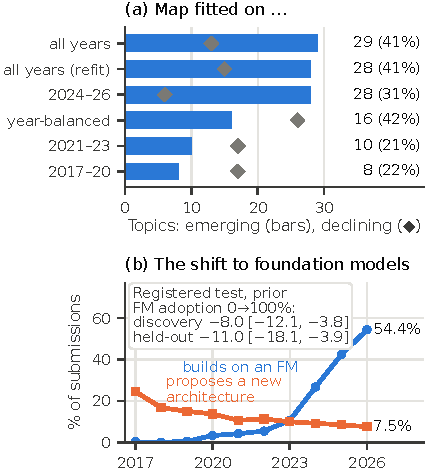
\includegraphics[width=0.62\textwidth]{figs/fig2_field.pdf}
  \caption[Emerging topics by fitting window, and the shift to foundation models]{(a) Emerging (bars) and declining
  (grey diamonds) topics on topic maps fitted on different years, for the same 43,480 papers. Labels at right show the
  number of emerging topics and, in brackets, the share of 2024--2026 papers in them (22.3\% on the 2017--2020 map,
  40.9\% on the all-years map); `all years (refit)' uses another random seed. Topic size `predicts' two-year growth
  only on the all-years map (out-of-sample $R^2 = 0.28$ against $-$0.03; no paired test). (b) Share of submissions
  building on an FM (blue) and proposing a new architecture (orange), using contribution types assigned by the LLM,
  with the registered test inset (\lab{replicated}).}
  \label{fig:field}
\end{figure}

\subsection{Waves}
Author keywords need no topic map, and at their level waves are real: 17 of the 68 most frequent keywords are
\emph{waves}, which rose and fell, peaking in 2019--2024 with shares of at most half the peak both before it and in
2026 (Figure~\ref{fig:waves}; \lab{exploratory}).

\subsection{Emergence depends on hindsight}
A topic is called \emph{emerging} if its 2024--2026 share is at least three times its 2017--2020 share, and
\emph{declining} if its 2024--2026 share is at most a third of its 2017--2020 share. With the same papers and pipeline,
a map fitted on 2017--2020 finds 8 emerging topics and one fitted on all years finds 29 (Figure~\ref{fig:field}a;
\lab{exploratory}). Two causes combine, and they cannot be separated. The all-years map uses the future to describe the
past, like leakage in prediction \citep{kapoor2023leakage} and hindsight bias in judgement
\citep{fischhoff1975hindsight}: with 69\% of its papers in 2024--2026, it is in effect a present-day map. The early map,
for its part, cannot represent topics born after 2020. The two counts therefore bracket the number of emerging topics.

The registered tests of whether a topic's contribution mix changes as it grows (H1a--c) were not supported on the
all-years map (Table~\ref{tab:verdicts}). On the early map, the method and measurement estimates point the predicted
way, so whether topics show such a life cycle also depends on how topics are defined.

\subsection{What lasts: the shift to foundation models}
The FM share rose every year from 2018 (Figure~\ref{fig:field}b). Prior FM adoption is associated with fewer
new-architecture papers (H1d): from 0 to 100\% adoption the difference is $-$7.98\,pp [$-$12.14, $-$3.82] in discovery
and $-$11.0 [$-$18.1, $-$3.9] on held-out papers (\lab{replicated}). The association may also run the other way. The
test for a parallel shift towards empirical or evaluation papers (H1e) is inconclusive ($-$0.63 [$-$3.64, +2.38]). The
pattern matches accounts of NLP's paradigm shifts \citep{gururaja2023build,saphra2024first,pramanick2023diachronic},
but lock-in \citep{hooker2021hardware}, efficient choice \citep{sutton2019bitter} and a bandwagon
\citep{fujimura1988molecular} predict it too. The field level therefore cannot separate the two routes.

% ===============================================================================================================
\section{Entry: who writes what (RQ2)}
\label{sec:entry}

This section asks what researchers write when they enter a topic, and whether they follow others into it as the
herding account implies.

\subsection{Newcomers propose methods}
The registered prediction was that newcomer papers, whose authors face the most uncertainty, would more often be
follow-on work: measurement papers that benchmark, collect data for or evaluate what others had proposed (H2b, H2c).
Newcomer papers make up 73\% of the 42,325 papers in 2019--2026 that have an author identifier. Compared with incumbent
papers, the difference in the share of method papers is +3.71\,pp [+2.61, +4.80] in discovery and +3.60 [+1.48, +5.71]
on held-out papers; for measurement papers it is $-$1.70 [$-$2.46, $-$0.93] and $-$2.10 [$-$3.35, $-$0.85]
(Table~\ref{tab:entry}, Figure~\ref{fig:entry}). Both contrasts are \lab{replicated}. The registered prediction thus
failed in the opposite direction, and the reversed hypotheses, registered before the held-out data were examined, were
supported on the held-out papers. All ten counted variants agree in sign, and the $t$-statistics (6.7 and $-$4.4) are
too large to be explained by the inflated false-positive rate reported in Section~\ref{sec:threats}. Team size accounts
for much of the measurement gap: with log team size as a control, the gap shrinks to $-$0.54 [$-$1.11, +0.04] in
discovery and $-$0.98 ($p = 0.10$) on held-out papers, whereas the method gap barely changes (+3.92 and +3.64).

\begin{table}[tb]
\centering
\footnotesize
\setlength{\tabcolsep}{3pt}
\renewcommand{\arraystretch}{1.1}
\begin{tabularx}{\textwidth}{@{}Y L{2.7cm} L{2.7cm} L{2.4cm}@{}}
\toprule
Contrast & Discovery [95\% CI] & Held-out [95\% CI] & Label \\
\midrule
Method paper & +3.71\newline[+2.61, +4.80] & +3.60\newline[+1.48, +5.71] & \lab{replicated} \\
Measurement paper & $-$1.70\newline[$-$2.46, $-$0.93] & $-$2.10\newline[$-$3.35, $-$0.85] & \lab{replicated} \\
Measurement paper, with log team size$^a$ & $-$0.54\newline[$-$1.11, +0.04] & $-$0.98\newline($p = 0.10$) &
\lab{registered variant} \\
\addlinespace
Method: returning topic newcomer $-$ incumbent$^b$ & +3.43\newline[+2.31, +4.55] & -- & \lab{exploratory} \\
Method: first-time team $-$ returning topic newcomer$^b$ & +0.92\newline[$-$0.44, +2.29] & -- & \lab{exploratory} \\
Distance from earlier ICLR work, own work excluded (percentile points) & +4.33\newline[+3.44, +5.22] & -- &
\lab{exploratory} \\
\addlinespace
Entry into hot topics: incumbent share, hot $-$ other topics$^c$ & $-$0.73\newline[$-$2.68, +1.22] & -- &
\lab{inconclusive} \\
\bottomrule
\end{tabularx}
\caption[Entry contrasts between newcomer and incumbent papers]{Entry contrasts: newcomer minus incumbent papers
unless the row names other profiles, in pp within topic and year. Held-out tests are one-sided. $^a$Registered
supplementary variant, outside the support rule. $^b$First-time team: no author has any earlier ICLR submission;
returning topic newcomer: an author has one, in another topic. $^c$H2a; no held-out test was registered.}
\label{tab:entry}
\end{table}

\subsection{Topic newcomers and first-time ICLR teams}
Newcomer papers split into those from first-time teams (26.3\% of papers; median team size 3) and those from returning
topic newcomers (46.7\%; median 5); incumbent papers make up the remaining 27.0\% (median 5). Returning topic newcomers
write method papers more often than incumbents (+3.43\,pp [+2.31, +4.55]) at the same median team size, and the
difference holds with team size controlled (+3.62). For first-time teams the difference is +4.35 [+2.82, +5.89], and
the interval for the gap between the two newcomer profiles includes zero (+0.92 [$-$0.44, +2.29]). All three contrasts
are \lab{exploratory}. The method surplus is therefore associated mainly with entering a topic, not with being new to
ICLR or with working in a small team, and it appears in every period, including before 2023.

The measurement gap behaves differently. For first-time teams it is accounted for by team size ($-$2.24 [$-$3.24,
$-$1.25] against incumbents, and +0.09 [$-$0.63, +0.80] with team size controlled); for returning topic newcomers part
of it remains ($-$1.47, and $-$0.81 [$-$1.46, $-$0.16] with team size controlled). The gap appears only in 2024--2026
(first-time teams against incumbents: $-$2.75 [$-$4.07, $-$1.44]). In the FM era, then, measurement papers are
concentrated among topic incumbents and larger teams. Team size is the only resource observed here; others, such as
compute, may also matter. NLP shows a parallel at the level of research trends, where tasks and methods lead and
datasets follow \citep{pramanick2023diachronic}.

\begin{figure}[tb]
  \centering
  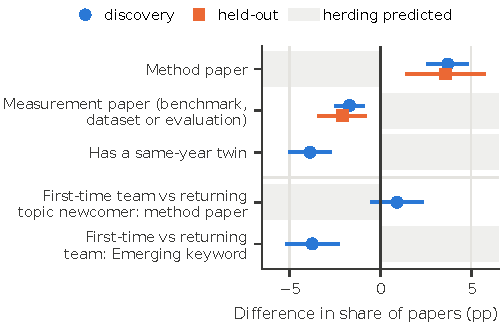
\includegraphics[width=0.72\textwidth]{figs/fig3_entry.pdf}
  \caption[Entry contrasts within topic and year]{Entry contrasts within topic and year (pp), with 95\% intervals:
  discovery (blue circles) and held-out (orange squares). Rows 1--2 compare newcomer with incumbent papers; they are
  registered and \lab{replicated}. Rows 3--5 are \lab{exploratory} (discovery only). Row 3 compares papers by returning
  topic newcomers with incumbent papers, with first-time teams entered separately and with contribution-type, FM and
  team-size controls. Row 4 compares first-time teams with returning topic newcomers, and row 5 compares first-time
  teams with returning teams (all teams with earlier ICLR submissions) on the use of young, rising Emerging keywords.
  Grey shading marks the side that the herding prediction expected.}
  \label{fig:entry}
\end{figure}

\subsection{Farther from earlier work}
Newcomer papers lie farther from earlier ICLR work than incumbent papers. Within topic and year the difference is
+5.90 percentile points [+4.95, +6.85]; it is +5.24 among method papers alone and +4.33 [+3.44, +5.22] when the
authors' own earlier papers are excluded from the reference set. Papers by returning topic newcomers are less likely
than incumbent papers to have a same-year \emph{twin}, an independent submission at cosine similarity $\geq 0.70$; with
first-time teams controlled separately, the difference in twin share is $-$3.86\,pp [$-$4.98, $-$2.74]. These results
are \lab{exploratory}. The follow-on prediction expects newcomer papers to lie closer to earlier work. Writing method
papers could itself be imitation of the venue's usual kind of paper, since three quarters of ICLR papers are method
papers, but newcomers' distance from earlier work argues against that reading. Neither contribution type nor embedding
distance measures originality; these results argue against newcomers following others but say nothing about whether
their work is more original.

\subsection{Later uptake of foundation models}
Among 2023--2026 papers in topics where 5--50\% of the previous year's papers built on FMs, the gap in FM-paper share
between first-time teams and returning topic newcomers is $-$4.58\,pp [$-$6.55, $-$2.60], widening to $-$14.71
[$-$19.82, $-$9.61] as adoption rises. For returning topic newcomers and incumbents the data show no clear difference.
First-time teams also list \emph{Emerging} keywords, which are young and rising, at a lower rate than teams with earlier
ICLR submissions; the difference is $-$3.74 [$-$5.14, $-$2.35]. Both results are \lab{exploratory}. Foundation models
thus spread through teams with earlier ICLR work, as absorptive capacity predicts \citep{cohen1990absorptive}. Network
diffusion predicts the same order, however, so this contrast cannot tell the routes apart.

\subsection{Flocking to hot topics}
Whether entrants crowd into hot topics remains open. The registered test (H2a), which compares the incumbent share in
hot and other topics, is inconclusive ($-$0.73 [$-$2.68, +1.22]), and no held-out test was registered for it. None of
the entry contrasts measured here favours the follow-on prediction.

% ===============================================================================================================
\section{The gate: crowd or record? (RQ3)}
\label{sec:gate}

This section asks whether acceptance at ICLR is associated with following the crowd or with staying close to the
authors' own earlier work. Table~\ref{tab:gate} and Figure~\ref{fig:gate} collect the tests. Of those in the figure,
crowding was registered, title style had been explored before registration and the remaining tests were found post hoc
in discovery; each held-out test was declared before any held-out estimate for its question was computed.

\subsection{Is following the crowd associated with acceptance?}
The registered crowding test (H3a) predicted a penalty for crowded topics, and it is uninformative. Per log unit of
crowding (the natural log of one plus the number of the topic's earlier papers), acceptance changes by $-$1.68\,pp
[$-$3.68, +0.32] in discovery and by $-$1.51 [$-$5.20, +2.19] on held-out papers, against an MDE80 of 4.8. The data
show no clear penalty or premium, although held-out premiums above +2.19\,pp per log unit lie outside the interval.
Whether the penalty is larger for method papers (H3b) could not be told ($-$0.36 [$-$1.51, +0.79]).

The clearest sign of imitation in the corpus is in title style. The share of titles that open with a short coined
name and a colon rose from 10.9\% in 2017 to 44.6\% in 2026. Within topic and year, with contribution-type, FM and
team-size controls, such branded titles are accepted 1.74\,pp [+0.37, +3.11] more often in discovery, but this estimate
is not a test, since title style had been explored before registration. The declared held-out test gives +1.76
[$-$0.82, +4.34] (one-sided $p = 0.089$); the held-out test is uninformative (below its MDE80 of 3.2), so the premium
remains \lab{exploratory}. Raw within-year gaps are larger (+3.3 in discovery and +4.0 on held-out papers); about half
of each gap is explained by topic, contribution type, FM use and team size. Titles can also be revised after the
decision, which could create such a premium.

FM papers are accepted 4.62\,pp more often [+2.79, +6.44], with no sign of a difference between late and early
adopters: the premium changes by +0.19 [$-$0.96, +1.34] per logit unit of the topic's prior FM adoption (that is, per
unit of its log-odds). Both results are \lab{exploratory}, and they fit efficient choice as well as imitation, if
review rewards it. A topic's \emph{edge} is its acceptance rate minus that of all other papers of the same year, using
topics of the 2017--2020 map. The edge persists but shrinks towards the mean: among discovery papers, the 2018--2022
edge predicts the 2024--2026 edge with slope 0.38 [0.18, 0.58]. The held-out test asks a related but different
question, namely whether the discovery edges for 2018--2022 predict the 2024--2026 edges of held-out papers; it gives a
slope of 0.60 [0.32, 0.88] and is \lab{held-out supported}. A favoured topic thus keeps only part of its edge, as
expected when decisions carry a large arbitrary component \citep{cortes2021inconsistency,beygelzimer2023has}.

Keyword timing shows at most weak associations, and it is treated as \lab{exploratory}: keyword popularity had been
explored against acceptance before registration, and both held-out intervals below include zero. On held-out papers,
\emph{Emerging} keywords (young and rising) are associated with higher acceptance than \emph{Mainstream} keywords (old
and flat), by +3.25 [$-$0.18, +6.69], and acceptance may fall after a keyword's share peaks ($-$5.2 [$-$11.1, +0.7];
$-$1.7 without the six keywords examined before this test was declared). Neither pattern shows the constant premium for
popular keywords that imitation would predict if review rewarded it.

\begin{table}[tb]
\centering
\footnotesize
\setlength{\tabcolsep}{3pt}
\renewcommand{\arraystretch}{1.1}
\begin{tabularx}{\textwidth}{@{}Y L{2.7cm} L{2.7cm} L{2.4cm}@{}}
\toprule
Contrast in acceptance & Discovery [95\% CI] & Held-out [95\% CI] & Label \\
\midrule
\multicolumn{4}{@{}l}{\textit{Referenced to the team's own record}} \\
Far jump: 10th percentile of \Fmax{} $-$ median & $-$5.44\newline[$-$7.10, $-$3.78] & $-$6.09\newline[$-$9.32,
$-$2.86] & \lab{held-out supported} \\
Same author, 0.1 closer in cosine similarity$^c$ & +0.55\newline[+0.21, +0.90] & +1.06\newline[+0.23, +1.89] &
\lab{held-out supported} \\
One topic insider vs none$^c$ & +3.42\newline[+1.18, +5.66] & +3.88\newline[+0.28, +7.47] & \lab{held-out supported} \\
\addlinespace
\multicolumn{4}{@{}l}{\textit{Referenced to others or the field}} \\
Crowding, per log unit$^a$ & $-$1.68\newline[$-$3.68, +0.32] & $-$1.51\newline[$-$5.20, +2.19] & \lab{uninformative} \\
Branded title$^b$ & +1.74\newline[+0.37, +3.11] & +1.76\newline[$-$0.82, +4.34] & \lab{exploratory} \\
Change in FM premium per logit unit of prior adoption & +0.19\newline[$-$0.96, +1.34] & -- & \lab{exploratory} \\
Topic edge 2018--22 \ra{} 2024--26, slope$^c$ & 0.38\newline[0.18, 0.58] & 0.60\newline[0.32, 0.88] & \lab{held-out
supported} \\
Emerging $-$ Mainstream keyword$^{b,c}$ & +2.67\newline[+0.76, +4.58] & +3.25\newline[$-$0.18, +6.69] &
\lab{exploratory} \\
Distance from earlier ICLR work: least-distant fifth $-$ middle fifth & $-$3.27\newline[$-$4.93, $-$1.60] &
$-$0.13\newline[$-$3.50, +3.25] & \lab{uninformative} \\
\bottomrule
\end{tabularx}
\caption[Acceptance contrasts at the gate]{Acceptance contrasts at the gate, in pp within topic and year (topic edges
and keywords: against the same year's other papers). Rows differ in population and unit, so their sizes are not
comparable. Held-out tests are one-sided. $^a$Registered (H3a); predicted a penalty; MDE80 4.8. $^b$Explored against
acceptance before registration. For titles the discovery estimate is not a test (held-out MDE80 3.2); for keywords it
is a declared post hoc test on a dimension already seen. $^c$Holm-adjusted $p$ across the six secondary held-out tests:
topic-edge slope 0.019, edge prediction 0.026, same-author closeness 0.026, insider 0.052, Emerging keywords 0.063,
same-author distance slope 0.22.}
\label{tab:gate}
\end{table}

\begin{figure}[tb]
  \centering
  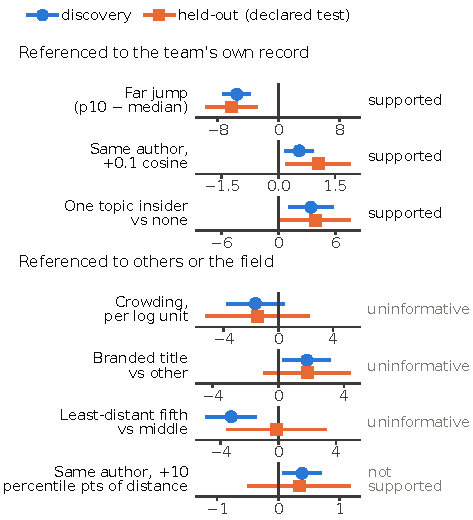
\includegraphics[width=0.72\textwidth]{figs/fig4_gate.pdf}
  \caption[Gate tests by reference point]{Gate tests by reference point: discovery estimates (blue circles) and
  declared held-out tests (orange squares), with 95\% intervals. The held-out verdict is shown at right: `supported' means
  \lab{held-out supported}; `uninformative' means not supported and below the test's MDE80; `not supported' marks a
  declared test without a registered MDE80, which is called inconclusive in the text. Each row has its own scale: pp for
  the far jump (closeness at its 10th percentile, p10, minus the median), the insider, the branded title and the
  least-distant fifth; pp per log unit for crowding; and pp per 0.1 cosine similarity and per 10 percentile points of
  distance for the two same-author slopes. Because the scales differ, compare verdicts rather than sizes.}
  \label{fig:gate}
\end{figure}

\subsection{What is acceptance associated with?}
The main pattern is the \emph{far jump}: the lower acceptance of papers far from the team's earlier work. Among
20,430 decided 2023--2026 papers with an experienced author, acceptance at the 10th percentile of closeness to the
team's own record is 5.44\,pp lower than at the median in discovery ($-$5.44 [$-$7.10, $-$3.78]) and 6.09\,pp lower on
held-out papers ($-$6.09 [$-$9.32, $-$2.86]), with power = 0.89. This was the primary test declared for the held-out
papers, and it is \lab{held-out supported}. Adjusted acceptance rises with closeness up to the fourth fifth of the
distribution. The far jump remains with a newcomer control ($-$5.0), although closeness is correlated with newcomer
status ($r = -0.57$).

Holding the author fixed, a paper 0.1 closer in cosine similarity to that author's earlier work is associated with
acceptance 0.55\,pp higher [+0.21, +0.90] in discovery and 1.06\,pp higher [+0.23, +1.89] on held-out papers. This
result is \lab{held-out supported} and survives a family-wise correction across the secondary tests. Controls for
newcomer status and for co-authors' experience change it little (+0.48 and +0.50), though unmeasured differences in
co-author quality could also bias it; a simulation run before the held-out test showed that such a confounder can
shift the estimate. In a related within-author comparison, on a paper in a topic new to them, the same author's
acceptance is 1.37\,pp lower ($-$1.37 [$-$2.74, $-$0.004]; author fixed effects, \lab{exploratory}).\footnote{Newcomer
papers as a whole have 10.2\,pp lower acceptance ($-$10.2 [$-$11.8, $-$8.7]) within topic and year
(\lab{exploratory}), but that gap mostly reflects who writes them: it shrinks once team size and the authors' ICLR
experience are controlled, and shrinks further within the same authors.}

Having one topic insider on the team, rather than none, is associated with acceptance 3.42\,pp higher [+1.18, +5.66] in
discovery and 3.88\,pp higher [+0.28, +7.47] on held-out papers, at fixed team size and number of experienced authors
(\lab{held-out supported}). The result does not survive the family-wise correction (Holm-adjusted $p = 0.052$), and
status explains it equally well: each additional insider adds only 0.58\,pp more than each additional experienced
author from another topic ($p = 0.16$; \lab{exploratory}).

Distance from earlier ICLR work as a whole gives uninformative results. In the same SPECTER2 vector space, papers in
the least-distant fifth differ from those in the middle fifth by $-$3.27 [$-$4.93, $-$1.60] in discovery but by $-$0.13
[$-$3.50, +3.25] on held-out papers, a test with power = 0.47. The within-author slope for distance from earlier ICLR
work was not supported either, and with no MDE80 available it is inconclusive. Of the distance-based tests, only the
associations with the team's own earlier work held up on held-out papers.
 % The Field

\chapter{Conclusions and Future Work}
\label{sec:conclusion}
\lhead{\emph{Chapter 5. Conclusions and Future Work}}  % page header

This report set out to test whether research in machine learning herds. It separated two ways in which a field can
conform, imitation of what others are doing and continuity with one's own record, and tested their predictions on ten
years of ICLR submissions at three levels: the field as a whole, entry to a topic and the acceptance decision. This
chapter first summarises the key findings (Section~\ref{sec:findings}). It then discusses what they mean for each
research question and how they relate to earlier work (Section~\ref{sec:discussion}), sets out the limitations
(Section~\ref{sec:limitations}) and suggests future work (Section~\ref{sec:future}).

\section{Summary of key findings}
\label{sec:findings}

At the level of the field (RQ1), keyword waves are real. Of the 68 most frequent author keywords, 17 rose and then fell
between 2019 and 2026 (\lab{exploratory}). The number of topics that appear to be emerging, however, depends on how the
topics are defined. The same papers give 8 emerging topics when the topic map is fitted on 2017--2020 and 29 when it is
fitted on all years (\lab{exploratory}). The one change that clearly lasted is the shift to foundation models: their
share of submissions rose from 0.3\% in 2017 to 54.4\% in 2026, and topics in which more papers built on FMs in the
previous year have fewer papers proposing a new architecture, by 8.0\,pp in discovery and 11.0\,pp on held-out papers
for a change from no adoption to full adoption (\lab{replicated}). The registered tests of whether a topic's mix of
contribution types changes as the topic grows were not supported.

At entry to a topic (RQ2), the registered herding prediction failed in the opposite direction. Papers by newcomers to a
topic are more often method papers than papers by incumbents, by 3.7\,pp in discovery and 3.6\,pp on held-out papers,
and less often measurement papers, by 1.7\,pp and 2.1\,pp (\lab{replicated}). The method surplus is linked to entering
the topic rather than to being new to ICLR, since researchers who already had ICLR papers in other topics show it as
well, and it appears in every period, including the years before 2023 (\lab{exploratory}). Much of the measurement gap
goes with team size, and in 2024--2026 measurement papers are concentrated among incumbents and larger teams. Newcomer
papers also lie farther from earlier ICLR work, and first-time ICLR teams take up foundation models and young, rising
keywords later than teams with an ICLR record (\lab{exploratory}). Whether entrants flock to hot topics could not be
decided (\lab{inconclusive}).

At the acceptance decision (RQ3), the registered test found no detectable penalty or premium for papers in crowded
topics, but the test could not rule out effects smaller than about 5\,pp per log unit (\lab{uninformative}). Branded
titles spread from 10.9\% to 44.6\% of titles and carry a small premium in discovery, which the held-out test was too
weak to confirm (\lab{exploratory}). The associations that held up on held-out papers all involve the team's own
earlier work. Papers far from it are accepted 5.4\,pp less often in discovery and 6.1\,pp less often on held-out
papers; for the same author, a paper closer to their earlier work is accepted more often; and a team with one topic
insider is accepted more often than a team with none (all \lab{held-out supported}, although the insider result does
not survive a family-wise correction). A topic that was favoured at review in 2018--2022 kept only part of its
advantage in 2024--2026 (\lab{held-out supported}). FM papers are accepted more often, by 4.6\,pp, and this premium did
not shrink as FMs spread within a topic, while the timing of keywords shows at most weak associations with acceptance
(both \lab{exploratory}).

\section{Discussion}
\label{sec:discussion}

\subsection{Does machine learning herd?}

Table~\ref{tab:routes} places each result under the route it fits. The field converged on foundation models, but
imitation, continuity, lock-in and efficient choice all predict that, so the field level cannot settle the question.
Where the two routes make different predictions, at entry and at the gate, the evidence leans towards continuity. The
registered herding predictions for entry failed or were inconclusive, and the registered crowding test at the gate was
uninformative. Every result that replicated at the gate is referenced to the team's own record, with one exception:
the persistence of topic edges, which fits imitation of past acceptance and regression to the mean in a noisy review
process equally well. The conformity that can be detected at ICLR is a pull towards a record rather than towards what
others are doing.

\begin{table}[tb]
\centering
\footnotesize
\setlength{\tabcolsep}{3pt}
\renewcommand{\arraystretch}{1.15}
\begin{tabularx}{\textwidth}{@{}L{2.3cm} Y Y@{}}
\toprule
 & Entry (what is written) & Gate (acceptance) \\
\midrule
\multicolumn{3}{@{}p{\textwidth}@{}}{\textbf{Field}, both routes: convergence on foundation models (\lab{replicated}),
also predicted by lock-in and efficient choice.} \\
\midrule
\textbf{Imitation} (others, now) & Follow-on prediction reversed (\lab{replicated}); newcomers farther from earlier
work and fewer twins for returning topic newcomers (\lab{exploratory}); flocking \lab{inconclusive}. & No detectable
crowding premium (\lab{uninformative}); branded titles: small premium, held-out test too weak (\lab{exploratory}).
Also fit a rival: topic edges partly kept (\lab{held-out supported}); no change in the FM premium; weak keyword timing
(\lab{exploratory}). \\
\midrule
\textbf{Continuity} (a record) & Incumbents write more measurement papers (\lab{replicated}; much of it with team size);
foundation models spread through teams with an ICLR record, as diffusion also predicts (\lab{exploratory}). & Lower
acceptance far from the team's record; higher for the same author's closer work and with a topic insider
(\lab{held-out supported}; status and expertise fit too). \\
\bottomrule
\end{tabularx}
\caption[Results by route and level]{Where conformity shows, by route and level. The table summarises
Chapter~\ref{sec:results} and adds no new estimates.}
\label{tab:routes}
\end{table}

This answer needs two qualifications. First, the absence of a detectable crowding premium does not rule out a
bandwagon. \citet{abrahamson1993institutional} showed that bandwagons can spread even when adopting brings no gain, and
the spread of branded titles may be such a case. Second, the record-side results at the gate fit continuity, but they
do not single it out. The next subsections take each research question in turn.

\subsection{The field: trends and hindsight}

The hindsight result speaks to a common practice in the history of research fields. Studies of PNAS, computational
linguistics and AI research have fitted one topic model to all years and then read trends from it
\citep{griffiths2004finding,hall2008studying,anderson2012towards,klinger2020narrowing}. The present results show that,
with the papers and the pipeline held fixed, the choice of fitting years alone can change the count of emerging topics
by a factor of more than three. This turns a concern raised in principle by \citet{leydesdorff2002dynamic} and
\citet{rotolo2015what} into a measured difference, and it adds the time window to the list of analysis choices that a
multiverse analysis would vary \citep{steegen2016increasing}. It also fits with recent work that tests signals of
emergence using only earlier data \citep{khanbayov2026topical}. The comparison is a bracket, not a correction: the
early map cannot see topics that appeared after 2020, so neither count is the true number.

The shift to foundation models is the clearest case of convergence in the corpus, and it matches the accounts of
paradigm shifts in NLP \citep{gururaja2023build,saphra2024first} and the concern about homogenisation around shared
models \citep{bommasani2021opportunities}. It is also what one would expect if general methods that scale with
computation simply work better \citep{sutton2019bitter}. Because both routes and both of these readings predict it,
the shift by itself says little about herding. This is the reason the report turned to entry and to the gate.

\subsection{Entry: who brings what}

The entry results run against the picture of the newcomer that underlies the herding account. In cascade models, the
person with the least information follows those who chose before them \citep{bikhchandani1992theory,banerjee1992simple}.
At ICLR, researchers new to a topic are the ones who more often propose methods, and their papers lie farther from
earlier work. This fits the literature on outsiders, which finds that people from the margin of a field more often
bring solutions and new ideas \citep{jeppesen2010marginality,zeng2021fresh,azoulay2019does}. The present results add
one detail that earlier work did not measure: the type of contribution. Newcomers bring methods, and incumbents and
larger teams write more of the benchmarks and evaluations. This is consistent with the finding that ML relies on a
small number of benchmark datasets \citep{koch2021reduced}, and with the observation in NLP that tasks and methods lead
while datasets follow \citep{pramanick2023diachronic}. A method paper is not necessarily an original one, however, so
these results say who proposes methods, not whose work is more novel.

First-time teams took up foundation models later than teams with earlier ICLR work. This fits absorptive capacity,
the idea that new knowledge is taken up by those who already hold related knowledge \citep{cohen1990absorptive}. It
fits network diffusion equally well \citep{coleman1957diffusion,rogers2003diffusion}, so it cannot separate the routes.
It does, however, contradict the idea that the newest entrants rush to whatever is fashionable. Half of the first
authors of LLM papers on arXiv in 2023 were new to LLM research \citep{movva2024topics}, but at ICLR, teams new to the
venue did not lead the adoption of foundation models.

\subsection{The gate: crowd or record}

The strongest result at the gate is the far jump: papers far from the team's earlier work are accepted less often.
This extends the pivot penalty, in which larger moves away from one's own past work go with lower impact and lower
publication success \citep{hill2025pivot}, to the accept or reject decision of an ML venue under double-blind review,
with every rejected paper in view. It also fits the finding that innovative research strategies are riskier
\citep{foster2015tradition}. The shape of the association matters: acceptance rises with closeness up to the fourth
fifth of the distribution and then levels off, so leaving one's record is associated with lower acceptance, but staying
very close brings no further gain. This reading suggests a threshold rather than a reward for repetition.

Several explanations fit these results, and the data cannot separate them. Continuity is one. Expertise is another:
reviewers may judge work from a team that knows the area as stronger, and with reason, as grant reviewers are both
biased towards and better informed about work in their own area \citep{li2017expertise}. Status is a third.
Cumulative advantage favours those already recognised \citep{merton1968matthew}, famous authors fare better when
reviewers can see them \citep{tomkins2017reviewer}, and preprints can reveal authors under double-blind review
\citep{bharadhwaj2020deanonymization}; at ICLR, a prestige gap has been tested with a pre-registered out-of-sample test
\citep{ibrahim2026bias}. The insider result is a good example. One insider on the team goes with higher acceptance,
which matches the chaperone effect \citep{sekara2018chaperone} and the finding that senior expertise offsets the
disadvantage of newcomers \citep{biliotti2024breaking}. But each additional insider adds little more than each
additional experienced author from another topic, so a proven record in general may matter more than knowledge of the
specific topic.

On the side of imitation, the gate shows little. The registered crowding test was too weak to detect effects of a few
points, which is consistent with the high level of noise in ML review \citep{cortes2021inconsistency,
beygelzimer2023has}. Topic edges persist only in part, which noise also predicts, although differences between research
areas in how reviewers score papers are a rival account \citep{xu2026reviewer}. Together with a randomised trial that
found no herding among reviewers in discussions \citep{stelmakh2023large}, the results give little support to the idea
that ICLR review rewards following the crowd. Whether evaluators penalise novelty remains contested
\citep{boudreau2016looking,teplitskiy2022is}, and the present results do not settle it: the penalty found here is for
distance from the team's own work, not for distance from the field, and the test of distance from earlier ICLR work as
a whole was uninformative.

\subsection{Why the distinction matters}

The two routes carry different risks for a field. Imitation can discard private information and leave a consensus
that rests on little evidence and breaks easily \citep{bikhchandani1992theory,banerjee1992simple}. Continuity trades
long-run exploration for short-run competence \citep{march1991exploration}, and choices that are safe for each
researcher can make a whole field explore less \citep{rzhetsky2015choosing}. A field that looks herded may in fact
conform by continuity, and a diagnosis of fads would then point to the wrong problem. Acceptance is also only a
short-run outcome. During the previous shift in ML, researchers who stayed close to their own record had lower later
impact \citep{bao2025persistence}, so the work that is accepted and the work that matters later need not be the same. For those who write the history of ML and NLP, the results suggest a simple check: before reading trends from a
topic model, refit it on early years and see which trends remain.

\section{Limitations}
\label{sec:limitations}

All results are associations at one venue, and none measures what would change if a researcher chose a different
topic, team, title or type of contribution. The held-out papers share conference years, reviewers and authors with the
discovery papers. The held-out tests therefore guard against overfitting by the analyst, but not against patterns that
are specific to a year or a pool of reviewers, and a supported held-out test confirms the direction of an association
rather than its size. The standard errors may also be too small: under one simulated null, the main entry tests gave a
significant result 12.6\% and 10.0\% of the time at a nominal 5\% level.

The framework of the report was built partly after the analysis. The distinction between imitation and continuity was
drawn up after the registered and declared tests had run, and the predictions of continuity were written afterwards.
The record-side results at the gate were found post hoc. Two of the three rest on secondary held-out tests, and the
insider result does not survive a family-wise correction. Keyword popularity and title style had been explored against
acceptance before registration.

The measures have their own limits. Contribution and FM labels come from an LLM. They were consistent across two runs,
but they were checked by hand only by the author, on 100 papers, about 20 of which were borderline, and there is no
measure of agreement with a second human coder. A method paper is a type of contribution, not a measure of novelty, and
distance in an embedding space is not originality. Entry status counts ICLR submissions only, and the change in author
identifiers in 2021 hides earlier histories, which pulls the entry contrasts towards zero. Some abstracts and titles
are final versions written after the decision; code links were removed for discovery papers, but titles could not be
corrected. Withdrawn papers are left out of the acceptance tests. Finally, the hindsight comparison is a bracket,
because the topic maps differ in the papers they are fitted on as well as in their time window.

\section{Future work}
\label{sec:future}

The most direct next step is to separate status from continuity. If the record-side associations reflect status, they
should be stronger where a preprint identifies the authors before review, which is how \citet{ibrahim2026bias} found
prestige to operate. Running this test would require a new declaration before any outcome is read, as the protocol of
this report requires.

The labels also need a human check that does not depend on one person. Two coders labelling the same random sample
independently would give agreement between humans and between humans and the LLM, and would show whether the
borderline cases change the entry results. A related question is what newcomers' method papers contain: whether they
propose new ideas or adapt existing ones to a new topic.

Several open questions could be answered with more data. Whether entrants flock to hot topics remains unsettled, and a
registered held-out test with enough power could settle it. Linking submissions to their later citations would show
whether the work that is accepted more often is also the work that has lasting impact, as the persistence results of
\citet{bao2025persistence} suggest it may not be. Withdrawn papers and the text of reviews could show whether the gate
also selects through withdrawal and what reviewers object to in papers that move far from their authors' earlier work.
Data on compute or institutions could show whether the concentration of measurement papers among incumbents reflects
resources other than team size.

Finally, the design could be repeated at other ML and NLP venues, such as NeurIPS or ACL, to see whether the findings
are specific to ICLR. Refitting topic maps on early years and using predictors measured only from the past could also
become a routine check for claims about research trends.

\section{Closing remarks}

Machine learning is easy to describe as a field that chases fashions, and its keyword waves and the rapid spread of
foundation models seem to confirm it. When the herding account is tested where it makes distinct predictions, however,
it finds little support at ICLR. Newcomers to a topic bring methods rather than follow-on work, and acceptance shows
no detectable association with following the crowd. What acceptance is associated with, instead, is staying close to
the team's own earlier work. Whether that reflects expertise, status or the value of continuing a line of
work is the main question this report leaves open.
 % Entry

\chapter{The Gate: Crowd or Record?}
\label{sec:gate}
\lhead{\emph{Chapter 6. The Gate}}  % page header

This chapter asks whether acceptance at ICLR favours papers that follow the crowd or papers anchored to their authors'
own earlier work.

\section{Is following the crowd associated with acceptance?}
Table~\ref{tab:gate} and Figure~\ref{fig:gate} collect the tests at the gate. Of those in the figure, crowding was
registered, title style had been explored before registration and the remaining tests were found post hoc in
discovery; each held-out test was declared before any held-out estimate for its question was computed.

The registered crowding test predicted a penalty for crowded topics, and it is uninformative. Per log unit of crowding
(the natural log of one plus the number of the topic's earlier papers), acceptance changes by $-$1.68\,pp [$-$3.68,
+0.32] in discovery and by $-$1.51 [$-$5.20, +2.19] on held-out papers, against an MDE80 of 4.8. In short, the data show no clear penalty or premium, although held-out premiums above +2.19\,pp per log unit lie outside the interval.

The clearest sign of imitation in the corpus is in title style. The share of titles that open with a short coined
name and a colon rose from 10.9\% in 2017 to 44.6\% in 2026. Within topic and year, with contribution-type, FM and
team-size controls, such branded titles are accepted 1.74\,pp [+0.37, +3.11] more often in discovery, but this estimate
is not a test, since title style had been explored before registration. The declared held-out test gives +1.76
[$-$0.82, +4.34] (one-sided $p = 0.089$); the held-out test is uninformative (below its MDE80 of 3.2), so the premium
remains \lab{exploratory}. Raw within-year gaps are larger (+3.3 in discovery and +4.0 on held-out papers); about half
of each gap is explained by topic, contribution type, FM use and team size. Titles can also be revised after the
decision, which could create such a premium.

FM papers are accepted 4.62\,pp more often [+2.79, +6.44], with no sign of a difference between late and early adopters: the premium changes by +0.19 [$-$0.96, +1.34] per logit unit of the topic's prior FM adoption (that is,
per unit of its log-odds). Both results are \lab{exploratory}, and they fit efficient choice as well as imitation, if
review rewards it. A topic's \emph{edge} is its acceptance rate minus that of all other papers of the same year, using
topics of the 2017--2020 map. The edge persists but shrinks towards the mean: among discovery papers, the 2018--2022
edge predicts the 2024--2026 edge with slope 0.38 [0.18, 0.58]. The held-out test asks a related but different
question, namely whether the discovery edges for 2018--2022 predict the 2024--2026 edges of held-out papers; it gives a
slope of 0.60 [0.32, 0.88] and is \lab{held-out supported}. A favoured topic thus keeps only part of its edge, as
expected when decisions carry a large arbitrary component \citep{cortes2021inconsistency,beygelzimer2023has}.

Keyword timing shows at most weak associations, and we treat it as \lab{exploratory}: keyword popularity had been
explored against acceptance before registration, and both held-out intervals below include zero. On held-out papers,
\emph{Emerging} keywords (young and rising) are associated with higher acceptance than \emph{Mainstream} keywords (old
and flat), by +3.25 [$-$0.18, +6.69], and acceptance may fall after a keyword's share peaks ($-$5.2 [$-$11.1, +0.7];
$-$1.7 without the six keywords examined before this test was declared). Neither pattern shows the constant premium for
popular keywords that imitation would predict if review rewarded it.

\begin{table}[tb]
\centering
\footnotesize
\setlength{\tabcolsep}{3pt}
\renewcommand{\arraystretch}{1.1}
\begin{tabularx}{\textwidth}{@{}Y L{2.7cm} L{2.7cm} L{2.4cm}@{}}
\toprule
Contrast in acceptance & Discovery [95\% CI] & Held-out [95\% CI] & Label \\
\midrule
\multicolumn{4}{@{}l}{\textit{Referenced to the team's own record}} \\
Far jump: 10th percentile of \Fmax{} $-$ median & $-$5.44\newline[$-$7.10, $-$3.78] & $-$6.09\newline[$-$9.32,
$-$2.86] & \lab{held-out supported} \\
Same author, 0.1 closer in cosine similarity$^c$ & +0.55\newline[+0.21, +0.90] & +1.06\newline[+0.23, +1.89] &
\lab{held-out supported} \\
One topic insider vs none$^c$ & +3.42\newline[+1.18, +5.66] & +3.88\newline[+0.28, +7.47] & \lab{held-out supported} \\
\addlinespace
\multicolumn{4}{@{}l}{\textit{Referenced to others or the field}} \\
Crowding, per log unit$^a$ & $-$1.68\newline[$-$3.68, +0.32] & $-$1.51\newline[$-$5.20, +2.19] & \lab{uninformative} \\
Branded title$^b$ & +1.74\newline[+0.37, +3.11] & +1.76\newline[$-$0.82, +4.34] & \lab{exploratory} \\
Change in FM premium per logit unit of prior adoption & +0.19\newline[$-$0.96, +1.34] & -- & \lab{exploratory} \\
Topic edge 2018--22 \ra{} 2024--26, slope$^c$ & 0.38\newline[0.18, 0.58] & 0.60\newline[0.32, 0.88] & \lab{held-out
supported} \\
Emerging $-$ Mainstream keyword$^{b,c}$ & +2.67\newline[+0.76, +4.58] & +3.25\newline[$-$0.18, +6.69] &
\lab{exploratory} \\
Distance from earlier ICLR work: least-distant fifth $-$ middle fifth & $-$3.27\newline[$-$4.93, $-$1.60] &
$-$0.13\newline[$-$3.50, +3.25] & \lab{uninformative} \\
\bottomrule
\end{tabularx}
\caption[Acceptance contrasts at the gate]{Acceptance contrasts at the gate, in pp within topic and year (topic edges
and keywords: against the same year's other papers). Rows differ in population and unit, so their sizes are not
comparable. Held-out tests are one-sided. $^a$Registered; predicted a penalty; MDE80 4.8. $^b$Explored against
acceptance before registration. For titles the discovery estimate is not a test (held-out MDE80 3.2); for keywords it
is a declared post hoc test on a dimension already seen. $^c$Holm-adjusted $p$ across the six secondary held-out tests:
topic-edge slope 0.019, edge prediction 0.026, same-author closeness 0.026, insider 0.052, Emerging keywords 0.063,
same-author distance slope 0.22.}
\label{tab:gate}
\end{table}

\begin{figure}[tb]
  \centering
  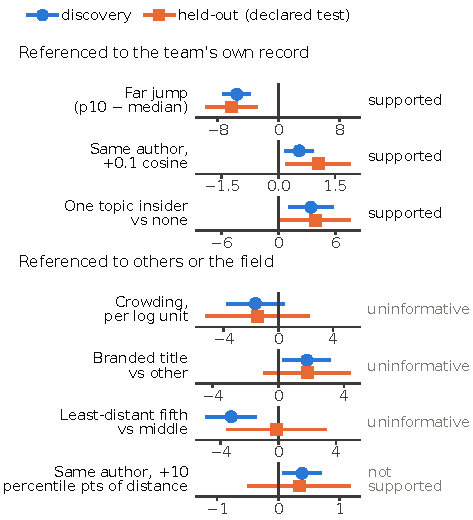
\includegraphics[width=0.72\textwidth]{figs/fig4_gate.pdf}
  \caption[Gate tests by reference point]{Gate tests by reference point: discovery estimates (blue circles) and
  declared held-out tests (orange squares), with 95\% intervals. The held-out verdict is shown at right: `supported' means
  \lab{held-out supported}; `uninformative' means not supported and below the test's MDE80; `not supported' marks a
  declared test without a registered MDE80, which we call inconclusive. Each row has its own scale: pp for the far
  jump (closeness at its 10th percentile, p10, minus the median), the insider, the branded title and the least-distant
  fifth; pp per log unit for crowding; and pp per 0.1 cosine similarity and per 10 percentile points of distance for
  the two same-author slopes. Because the scales differ, compare verdicts rather than sizes.}
  \label{fig:gate}
\end{figure}

\section{What is acceptance associated with?}
The main pattern is the \emph{far jump}: the lower acceptance of papers far from the team's earlier work. Among
20,430 decided 2023--2026 papers with an experienced author, acceptance at the 10th percentile of closeness to the
team's own record is 5.44\,pp lower than at the median in discovery ($-$5.44 [$-$7.10, $-$3.78]) and 6.09\,pp lower on
held-out papers ($-$6.09 [$-$9.32, $-$2.86]), with power = 0.89. This was the primary test declared for the held-out
papers, and it is \lab{held-out supported}. Adjusted acceptance rises with closeness up to the fourth quintile. The far
jump remains with a newcomer control ($-$5.0), although closeness is correlated with newcomer status ($r = -0.57$).

Holding the author fixed, a paper 0.1 closer in cosine similarity to that author's earlier work is associated with
acceptance 0.55\,pp higher [+0.21, +0.90] in discovery and 1.06\,pp higher [+0.23, +1.89] on held-out papers. This
result is \lab{held-out supported} and survives a family-wise correction across the secondary tests. Controls for
newcomer status and for co-authors' experience change it little (+0.48 and +0.50), though unmeasured differences in
co-author quality could also bias it; a simulation run before the held-out test showed that such a confounder can
shift the estimate. In a related within-author comparison, on a paper in a topic new to them, the same author's
acceptance is 1.37\,pp lower ($-$1.37 [$-$2.74, $-$0.004]; author fixed effects, \lab{exploratory}).\footnote{Newcomer
papers as a whole have 10.2\,pp lower acceptance ($-$10.2 [$-$11.8, $-$8.7]) within topic and year
(\lab{exploratory}), but that gap mostly reflects who writes them: it shrinks once team size and the authors' ICLR
experience are controlled, and shrinks further within the same authors.}

Having one topic insider on the team, rather than none, is associated with acceptance 3.42\,pp higher [+1.18, +5.66] in
discovery and 3.88\,pp higher [+0.28, +7.47] on held-out papers, at fixed team size and number of experienced authors
(\lab{held-out supported}). The result does not survive the family-wise correction (Holm-adjusted $p = 0.052$), and
status explains it equally well: each additional insider adds only 0.58\,pp more than each additional experienced
author from another topic ($p = 0.16$; \lab{exploratory}).

Distance from earlier ICLR work as a whole gives uninformative results. In the same SPECTER2 embedding space, papers in
the least-distant fifth differ from those in the middle fifth by $-$3.27 [$-$4.93, $-$1.60] in discovery but by $-$0.13
[$-$3.50, +3.25] on held-out papers, a test with power = 0.47. The within-author slope for distance from earlier ICLR
work was not supported either, and with no MDE80 available it is inconclusive. Of the distance-based tests, only the
associations with the team's own earlier work held up on held-out papers.

\section{Interpretation}
These associations all involve closeness to the team's own earlier work, as continuity predicts, but expertise,
evaluator conservatism and visible status predict them as well \citep{li2017expertise,merton1968matthew}. Double-blind
review does not rule status out: where reviewers can see the authors, famous authors fare better
\citep{tomkins2017reviewer}, and preprints can reveal who wrote a paper \citep{bharadhwaj2020deanonymization}.

% ===============================================================================================================
 % The Gate

%\input{Chapters/Chapter7} % Discussion (withheld until supervisor feedback)

%\input{Chapters/Chapter8} % Conclusion (withheld until supervisor feedback)

%% ----------------------------------------------------------------
% Now begin the Appendices, including them as separate files

\addtocontents{toc}{\vspace{2em}} % Add a gap in the Contents, for aesthetics

% \appendix % Appendices of the full paper are not included in this draft

% \chapter{An Appendix}

Lorem ipsum dolor sit amet, consectetur adipiscing elit. Vivamus at pulvinar nisi. Phasellus hendrerit, diam placerat interdum iaculis, mauris justo cursus risus, in viverra purus eros at ligula. Ut metus justo, consequat a tristique posuere, laoreet nec nibh. Etiam et scelerisque mauris. Phasellus vel massa magna. Ut non neque id tortor pharetra bibendum vitae sit amet nisi. Duis nec quam quam, sed euismod justo. Pellentesque eu tellus vitae ante tempus malesuada. Nunc accumsan, quam in congue consequat, lectus lectus dapibus erat, id aliquet urna neque at massa. Nulla facilisi. Morbi ullamcorper eleifend posuere. Donec libero leo, faucibus nec bibendum at, mattis et urna. Proin consectetur, nunc ut imperdiet lobortis, magna neque tincidunt lectus, id iaculis nisi justo id nibh. Pellentesque vel sem in erat vulputate faucibus molestie ut lorem.

Quisque tristique urna in lorem laoreet at laoreet quam congue. Donec dolor turpis, blandit non imperdiet aliquet, blandit et felis. In lorem nisi, pretium sit amet vestibulum sed, tempus et sem. Proin non ante turpis. Nulla imperdiet fringilla convallis. Vivamus vel bibendum nisl. Pellentesque justo lectus, molestie vel luctus sed, lobortis in libero. Nulla facilisi. Aliquam erat volutpat. Suspendisse vitae nunc nunc. Sed aliquet est suscipit sapien rhoncus non adipiscing nibh consequat. Aliquam metus urna, faucibus eu vulputate non, luctus eu justo.

Donec urna leo, vulputate vitae porta eu, vehicula blandit libero. Phasellus eget massa et leo condimentum mollis. Nullam molestie, justo at pellentesque vulputate, sapien velit ornare diam, nec gravida lacus augue non diam. Integer mattis lacus id libero ultrices sit amet mollis neque molestie. Integer ut leo eget mi volutpat congue. Vivamus sodales, turpis id venenatis placerat, tellus purus adipiscing magna, eu aliquam nibh dolor id nibh. Pellentesque habitant morbi tristique senectus et netus et malesuada fames ac turpis egestas. Sed cursus convallis quam nec vehicula. Sed vulputate neque eget odio fringilla ac sodales urna feugiat.

Phasellus nisi quam, volutpat non ullamcorper eget, congue fringilla leo. Cras et erat et nibh placerat commodo id ornare est. Nulla facilisi. Aenean pulvinar scelerisque eros eget interdum. Nunc pulvinar magna ut felis varius in hendrerit dolor accumsan. Nunc pellentesque magna quis magna bibendum non laoreet erat tincidunt. Nulla facilisi.

Duis eget massa sem, gravida interdum ipsum. Nulla nunc nisl, hendrerit sit amet commodo vel, varius id tellus. Lorem ipsum dolor sit amet, consectetur adipiscing elit. Nunc ac dolor est. Suspendisse ultrices tincidunt metus eget accumsan. Nullam facilisis, justo vitae convallis sollicitudin, eros augue malesuada metus, nec sagittis diam nibh ut sapien. Duis blandit lectus vitae lorem aliquam nec euismod nisi volutpat. Vestibulum ornare dictum tortor, at faucibus justo tempor non. Nulla facilisi. Cras non massa nunc, eget euismod purus. Nunc metus ipsum, euismod a consectetur vel, hendrerit nec nunc.	% Appendix Title

%\input{Appendices/AppendixB} % Appendix Title

%\input{Appendices/AppendixC} % Appendix Title

\addtocontents{toc}{\vspace{2em}}  % Add a gap in the Contents, for aesthetics
\backmatter

%% ----------------------------------------------------------------
\label{Bibliography}
\lhead{\emph{Bibliography}}  % Change the left side page header to "Bibliography"
\bibliographystyle{unsrtnat}  % Use the "unsrtnat" BibTeX style for formatting the Bibliography
\bibliography{Bibliography}  % The references (bibliography) information are stored in the file named "Bibliography.bib"

\end{document}  % The End
%% ----------------------------------------------------------------